Cette section donne une idée basique de la structure et des éléments qui seront nécessaire au fonctionnement du système.
Ceci va permettre de faire des calculs préliminaires ainsi que de déterminer quels éléments critiques seront étudiés lors du choix
de solutions.

\section{Partie mobile}\label{sec:PartMob}
L'utilisation d'un moteur linéaire est obligatoire, il y a donc forcément un \gls{glider} dans le système. Le \gls{glider} n'est cependant
pas guidé dans son rail, il faut donc un guidage linéaire en plus qui aura un chariot pour pouvoir se fixer dessus. Une tige de matière
transparente devra être présente aussi pour faire office de pendule. Pour pouvoir réguler le système il faut pouvoir récupérer des variables
du système, dans ce cas-ci, la position linéaire et la position angulaire de la tige. Ceci signifie qu'il est nécessaire d'avoir des encodeurs
pour connaître ces valeurs. Il y aura donc l'ajout d'un encodeur angulaire sur la partie mobile ainsi que de la tête de lecture d'un encodeur
linéaire si ce dernier n'est pas déjà inclut dans le guidage linéaire choisit. Finalement, des pièces en aluminium sur mesure seront nécessaire
pour lier tous ces éléments entre eux.

\begin{figure}[H]
    \centering
    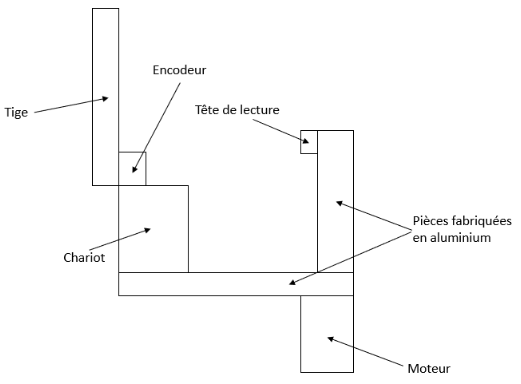
\includegraphics[width = 0.7\textwidth]{assets/figures/StructPrelim.svg}
    \caption{Structure préliminaire du système}
    \label{fig:StructPrelim}
\end{figure}